\section{Strengths and weaknesses}
	Summarizing, this document shows a vision-based tracking algorithm to be used by UAVs. This algorithm is able to target multiple objects based on their color. This last sentence is the main advantage if it's compared with other algorithms as CAMSHIFT's \cite{CAMSHIFT_FAST} \cite{CAMSHIFT_ENVIROMENT}  and so on. The bottle neck of color-based algorithm use to be the computational time, however, our implementation allows to UAV to process fastly the taken pictures. In both cases the algorithm processes faster than 40 pictures by second.
	The algorithm was tested on many simulations inside the V-REP application and using a variety of datasets provided by the GRVC. In both cases, estimation's error is less than a 10\% of the distance between the target and the camera.
	In parallel of the developing of the algorithm, we develop a cross-platform library in order to make the code easy to use, not only inside this project, but in many applications. Chapter 7 \ref{chap:c6_bovil} have a brief description of this library.
	
	% % TODO 666 ADD CITES!!
	
\section{Future Branches}
	In this section we propose some possible improvements for the algorithms or application's architecture.
	
	\subsection{Parallel Color Clustering}
	One of the bottle necks of the algorithm is the color clustering or color segmentation of the image. Every step of the algorithm requires to check every single pixel of the input images. This fragment of the algorithm is easily implementable under the parallel paradigm. Using the Graphic Processor Unit (GPU) instead of the Computer Processor Unit (CPU) it possible to increase the speed of the segmentation algorithm considerably \cite{GPU_CPU_performance} \cite{GPU_parallel_image_processing} \cite{GPU_enabled_parrallel}.
	GPU's cores are slower than general CPU's cores. However there are more cores in GPU than in CPU \ref{fig:gpu}, so parallelization in GPU can highly improve the global speed of the process.
		
	\begin{figure}[ph]
		\centering
		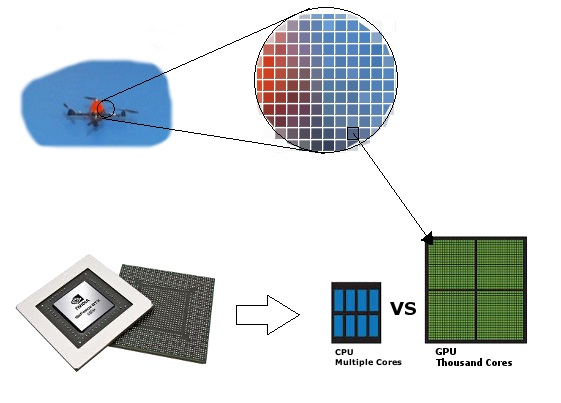
\includegraphics[width=0.7\linewidth]{../Images/c5/gpu}
		\caption{Parallelization}
		\label{fig:gpu}
	\end{figure}


	\subsection{Shape recognition}
	At the moment, the criteria of choosing the target is size and color. Nevertheless, where there are multiple possible targets in the scene it could confuse them or divide them if they are composed of more than one color. So shape recognition \cite{color_shape_object_recogn} \cite{Fast_object_recogn_shape} should be an useful tool to differentiate many objects once they were segmented.
	
	\begin{figure}[th]
		\centering
		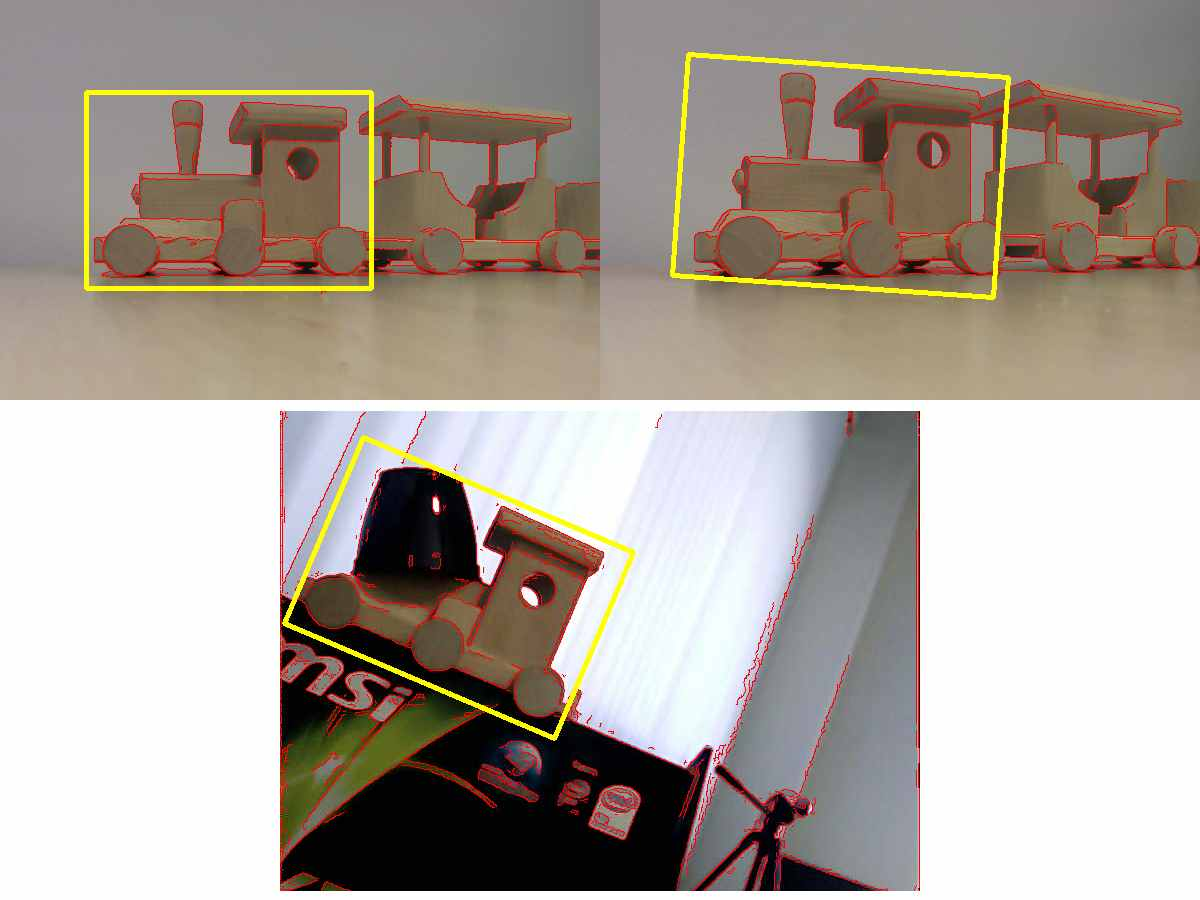
\includegraphics[width=0.6\linewidth]{../Images/c6/shape_recogn}
		\caption{Shape recognition}
		\label{fig:shape_recogn}
	\end{figure}
		
	\subsection{Higher Conscience}
	Finally another improvement (this one about the complete architecture of the software) is the addition of a higher conscience or AI that could arrange the amount of information and use it to improve the perception of the environment \cite{Multirate_sampled_uav} \cite{multi_uav_path_planning}.
	For example, storing the information about the geometrical position and speed of the targets associated with object recognition provided by algorithms from the image sensor sources can be used to make complex task planning \cite{task_allocation}.
	
	\subsubsection{Big Data}
	This term refers to any collection of datasets so large and complex that it becomes difficult to process using traditional data processing application. If the system is huge enough, it will be interesting design a right architecture for storing the data. There are many approaches\cite{Big_data_Ecosystem} \cite{Big_data_mapReduce} and solutions to prevent the system to collapse while searching information to make a decision.
	
	\begin{figure}[th]
		\centering
		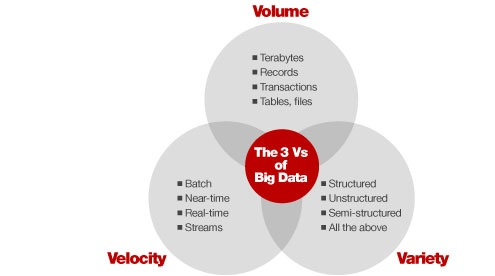
\includegraphics[width=0.7\linewidth]{../Images/c6/big_data}
		\caption{Big Data}
		\label{fig:big_data}
	\end{figure}
		
	\subsubsection{Cloud Computing}

	Dividing the process of the ground station into multiple servers (or computers) can improve the speed and robustness of the system. This concept (Cloud Computing) relies on sharing resources to achieve coherences over a network \ref{fig:cloud_computing}. It aims to maximizing the effectiveness of shared resources, not only dividing the process and resource, but doing int dynamically reallocating during the time. \cite{Cloud_computing}
	
	\begin{figure}[th]
		\centering
		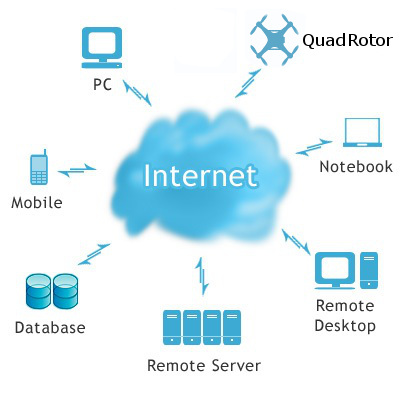
\includegraphics[width=0.7\linewidth]{../Images/c6/cloudcomputing}
		\caption{Cloud Computing}
		\label{fig:cloud_computing}
	\end{figure}

	
	
